\documentclass[11pt]{article}
%ACENTOS
\usepackage[utf8]{inputenc}
\def\figurename{Fig.}
\def\tablename{Tabla}
\def\refname{Referencias}
\setlength{\parskip}{1em}

%PAQUETES
\usepackage{amsfonts,amsmath,amssymb}    % need for subequations
\usepackage{amsmath,latexsym}
\usepackage{graphics,color}
\usepackage{graphicx}
\usepackage{algpseudocode}
\usepackage[most]{tcolorbox}
\usepackage{hyperref} %Para colocar direcciones Web
\usepackage{booktabs} % Tablas
\usepackage[thinc]{esdiff} % Derivadas

%MARGEN
\setlength\topmargin{-0.5in}
\addtolength\oddsidemargin{-0.5in}
\setlength{\textheight}{23cm}
\setlength{\textwidth}{16cm}

%VARIABLES
\newcommand{\N}{\mathbb N}
\newcommand{\Z}{\mathbb Z}
\newcommand{\R}{\mathbb R}
\newcommand{\C}{\mathbb C}
\providecommand{\norm}[1]{\lVert#1\rVert}
%COLORES
\newcommand{\rojo}[1]{\textcolor[rgb]{1.00,0.00,0.00}{#1}}
\newcommand{\azul}[1]{\textcolor[rgb]{0.00,0.00,1.00}{#1}}
\usepackage{empheq}

\documentclass[fleqn]{article}
\usepackage{amsmath}

\newcommand{\cajaverde}[2]{
    \begin{tcolorbox}[colframe=green!70!black, title=#1]
        % Contenido
        #2
    \end{tcolorbox}
} 
  
\begin{document}

\begin{center}
 \Large \underline {\\ \\Tarea 5: Mínimos cuadrados}
  \\
  \\
 \small  {Elaborado por Giselt Parra}\\ 
 \footnotesize{Domingo, 22 de Noviembre de 2020.}
\end{center}

Para abordar el problema a una solución si bien es cierto que la idea es conseguir los parámetros que se adecuen al modelo y den como resultado  valores cercanos a la data real minimizando el error entre ambas, como vector inicial se deben ingresar valores de tal manera que el modelo se encuentre lo suficientemente cerca a la solución adecuada. 

En un principio, para la asignación de los valores de los parámetros iniciales se tomó en cuenta la información general que se maneja y está disponible sobre el virus sin fijar restricciones en el rango de los parámetros para experimentar con mayor libertad dentro de cualquier valor mientras estuviera dentro de los valores permitidos siendo éstos parámetros proporciones, probabilidades y porcentajes. 

Los parámetros a estimar son los siguientes. Se explicará que información aporta cada uno de ellos y se toma en cuenta la información disponible que se tiene hasta el momento para hacer una primera estimación de manera intuitiva:

\begin{enumerate}
	\item[\textperiodcentered] \textbf {$\alpha$}: representado por un vector de dos elementos, tiempo de latencia y tiempo de incubación, ambos promedios de lo que representan respectivamente. Se puede establecer una diferencia entre ambos elementos dado a que el tiempo de latencia comprende en el periodo donde un individuo estuvo expuesto al virus y concluye en el momento donde puede contagiar a otros aún sin presentar síntomas mientras el periodo de incubación se considera así desde la exposición del individuo hasta que empieza a presentar los primeros cuadros clínicos de la infección, por lo que se suma el tiempo de latencia junto al periodo de tiempo donde es infeccioso hasta que presenta síntomas y por tanto, es mayor. De la información extraida por los organismos de salud el número de días que puede tomar un individuo en periodo de latencia es entre 5 y 14 días.
	
	
	\item[\textperiodcentered] \textbf {$\beta$}: representa la tasa de infección. Viene dada por un vector de tres componentes donde dicho valor variará dependiendo de las caracteristicas de la infección en la población. Se dividen en tres tasas por los siguientes compartimientos. $betaP$ para la tasa de infección en el casos de los presintomáticos, $betaT$ para el caso de la población que ya presenta síntomas del virus y $betaA$ para el caso de asintomáticos. Se podría considerar el parámetro con más peso dentro del estudio en el número de casos (y por consecuente de fallecimientos). La razón por la que se considera de esta manera es porque representa la probabilidad de que un individuo que pueda contagiar infecte a población susceptible y así se propaga el virus. Presenta una dificultad estimar este parámetro sobretodo en el caso de $betaA$ que considera cuando quien propaga el virus es un caso asintomático, al no presentar síntomas resulta más complicado contabilizar el número de casos de infección que pueda darse con esta caracteriztica, sin embargo, esto nos da una idea de que el valor de $betaA$ es mayor al de $betaT$ por la falta de medidas de precaución del individuo infectado así como de los posibles afectados.
	

	\item[\textperiodcentered] \textbf {$\gamma$}: al igual que los dos parámetros a expuestos, la tasa de recuperación se separa en el caso de sintómaticos al de asintomáticos. Estudios realizados indican que para los casos donde los individuos no presentaron síntomas, el tiempo de recuperación fue menor que el caso contrario con una diferencia grande en los casos más severos de casos sintomáticos.
	
	\item[\textperiodcentered] \textbf {$\pi$}: determina el número de casos en proporción de cuántos individuos presentarán los síntomas del virus.
	
	\item[\textperiodcentered] \textbf {$\kappa$}: representa la tasa de fatalidad del virus. 
	
	\item[\textperiodcentered] \textbf {$\eta$}: representa la tasa de protección donde se pasa de un estado susceptible a un estado no susceptible por unidad de tiempo.
	
	\item[\textperiodcentered] \textbf {$\delta$}: indica la proporción en el caso de los individuos recuperados vuelven a ser susceptibles. Para este estudio se asume que una vez recuperada una persona, no volverá al estado de susceptibilidad por lo que eventualmente en un largo periodo de tiempo se esperaria una disminucion en todos los valores que indiquen incremento de casos. Por tanto, el valor de delta se toma como cero.
\end{enumerate}

Al ejecutar el modelo dentro de la función $lsqcurvefit$ se obtuvieron los siguiente parámetros

\begin{center}
    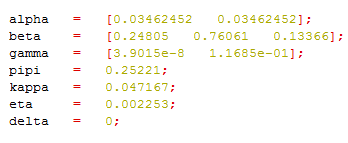
\includegraphics[keepaspectratio, width=8cm]{parametros.png}
    \caption{
    \\\alpha: alpha 
    \\\beta: beta
    \\\gamma: gamma
    \\\pi: pipi
    \\\kappa: kappa
    \\\eta: eta
    \\\delta: delta}
    
\end{center} 

dando como resultados esta estimación para el número acumulado de casos

\begin{center}
    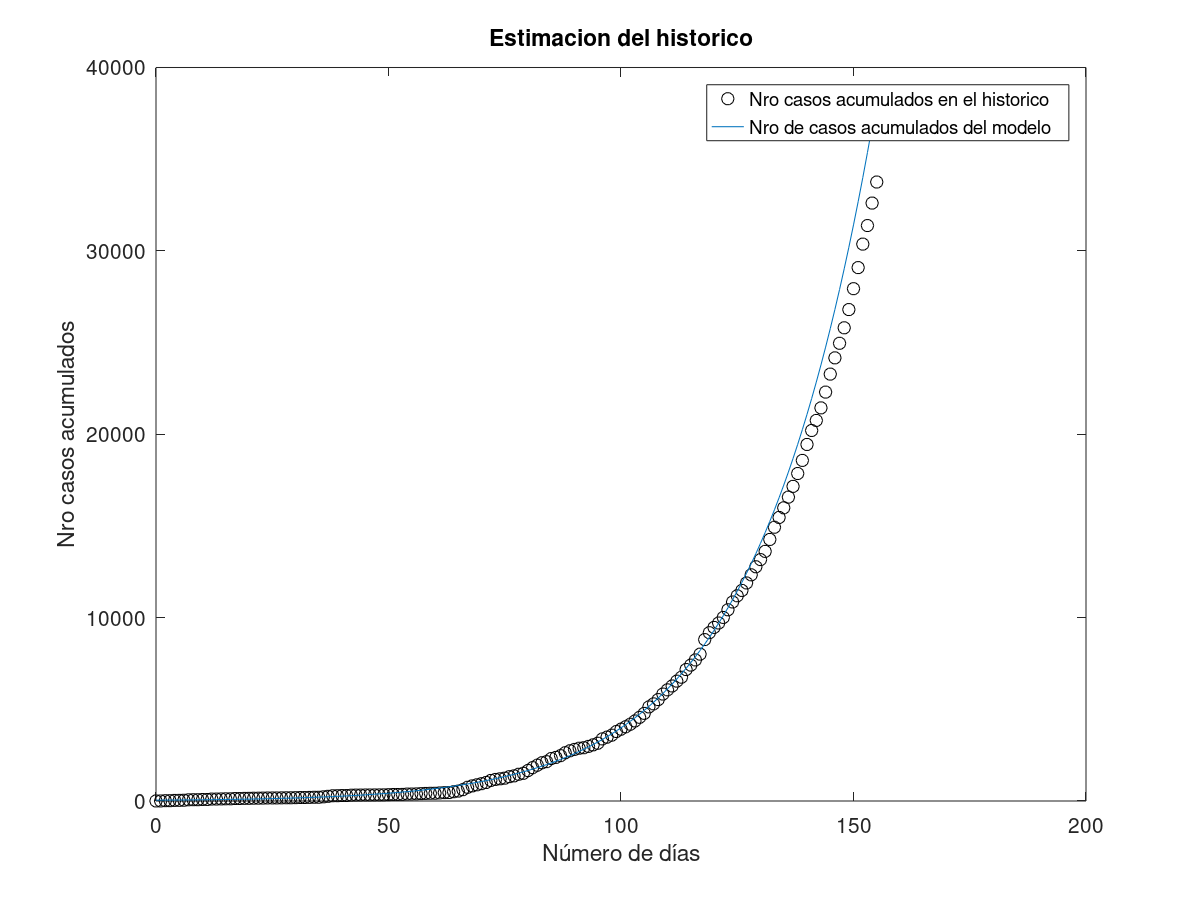
\includegraphics[keepaspectratio, width=12cm]{Funcion.png}
    \caption{\\}
\end{center}  

Respecto a la data histórica sobre los casos de fallecimiento se presentó el inconveniente de que los valores resultantes eran muy elevados en comparación a los datos a estimar.

\begin{center}
    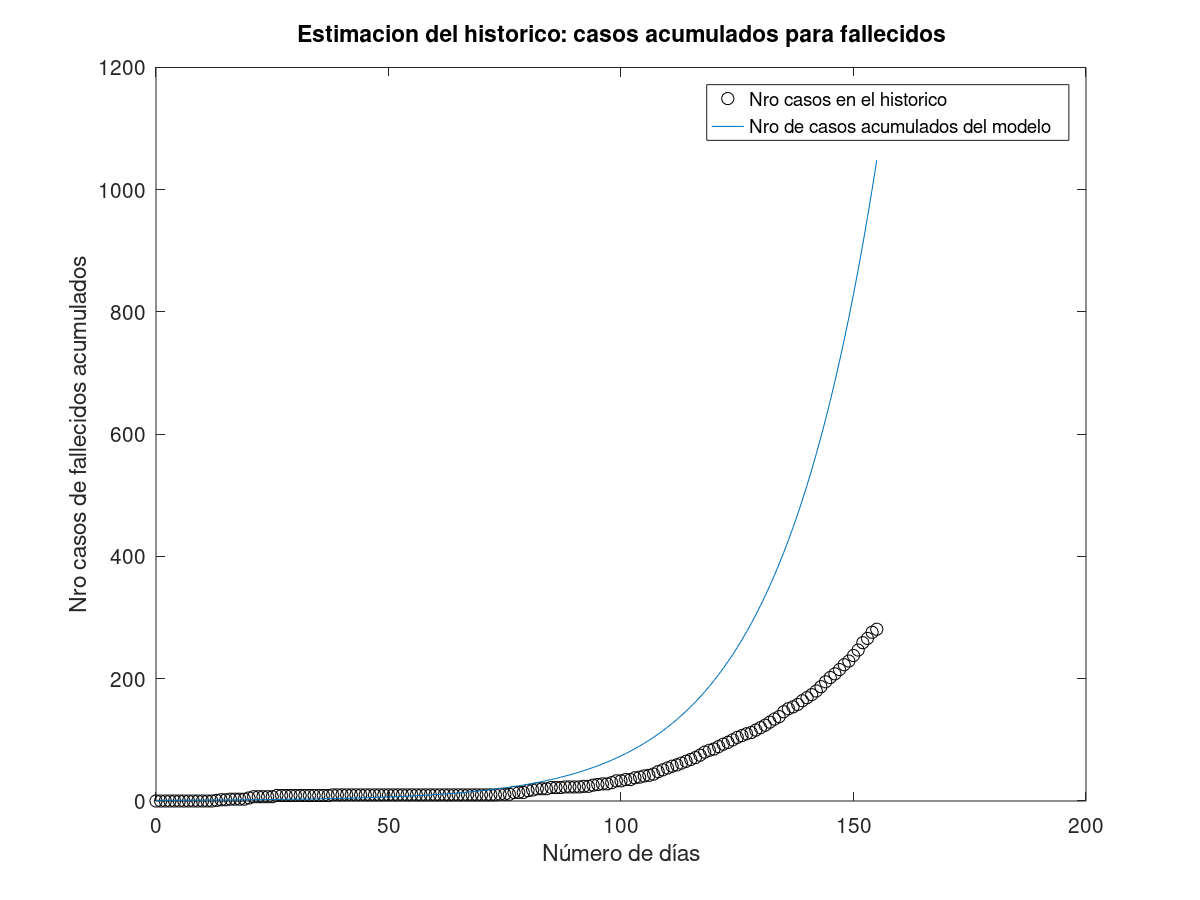
\includegraphics[keepaspectratio, width=12cm]{FuncionMortalidad.png}
    \caption{\\}
\end{center} 

Sin embargo, se confía en el valor del parámetro que indica la tasa de fatalidad del virus cuando se toma en cuenta el porcentaje de población que mayormente se encuentra susceptible y en un estado de exposición constante como son los adultosen edades comprendidas entre los 20 y 65 años, donde se llegó a un valor de tasa de mortalidad de $\kappa = 0.0245$ . Tomando en cuenta el número de casos acumulados, los valores para el historial de fallecidos con este parámetro modificado presenta un número razonable aunque sigue sin ser cercano al número real

\begin{center}
    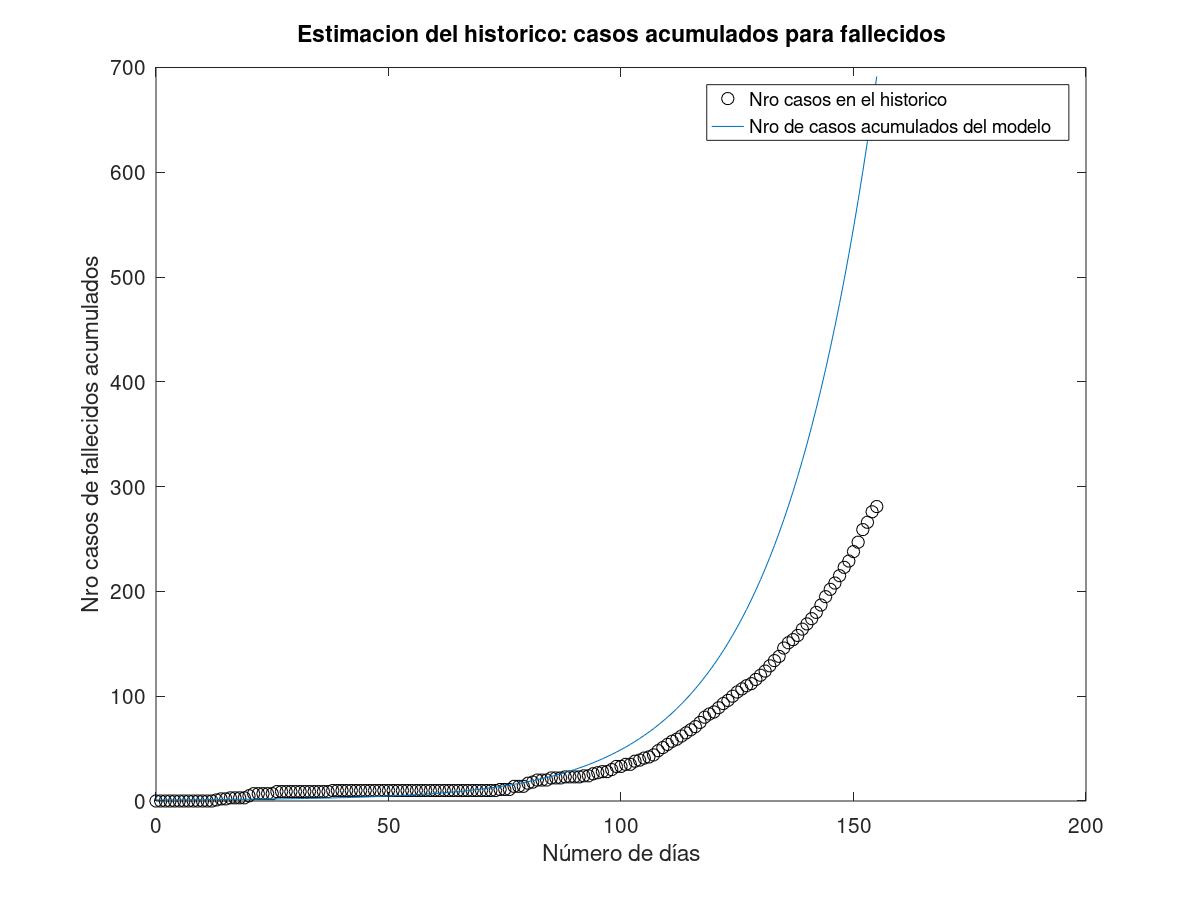
\includegraphics[keepaspectratio, width=12cm]{FuncionMortalidad2.png}
    \caption{\\Estimación de número de casos de fallecidos con $\kappa = 0.0245$ }
\end{center} 

Comentarios: Si se reduce el valor de la tasa de mortalidad a $\kappa = 0.0135$ resulta una estimación mucho más cercana a los datos de entrada obteniendo así un comportamiento parecido al resultante cuando se utiliza el valor de $kappa$ dado por el método $lsqcurvefit$. No obstante, a pesar de ser comentado esta modificación como una mejor aproximación a los datos reales, se está en desacuerdo en alterar estos valores con el propósito de aproximar mejor la data histórica, siendo un estudio de gran sensibilidad, el hacer esto implicaría restarle gravedad a un problema tan grave como es una pandemia.

\begin{center}
    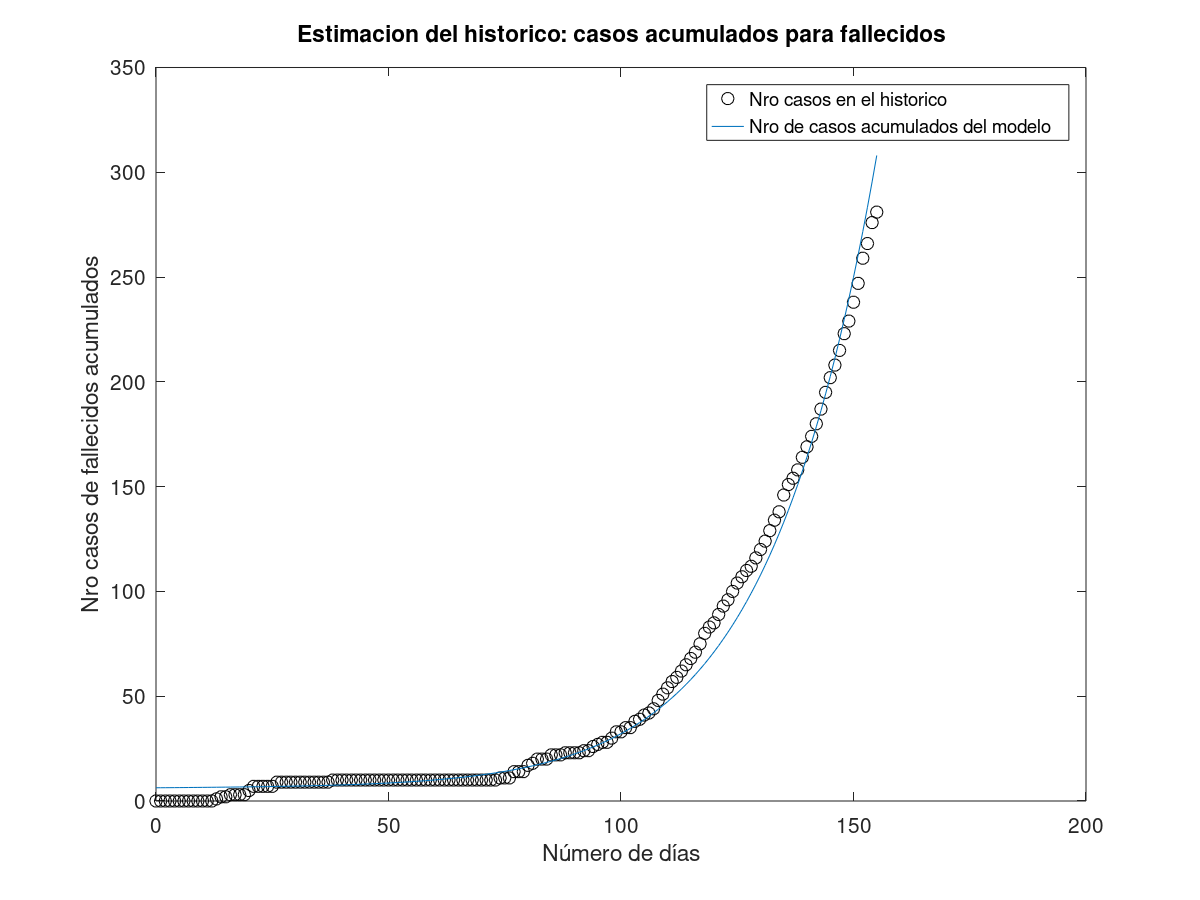
\includegraphics[keepaspectratio, width=12cm]{FuncionMortalidad3.png}
    \caption{\\Estimación de número de casos de fallecidos con $\kappa = 0.0135$ }
\end{center} 

\begin{center} \Large {Resultados y comportamiento de los compartimientos} \end{center}



\begin{center}
    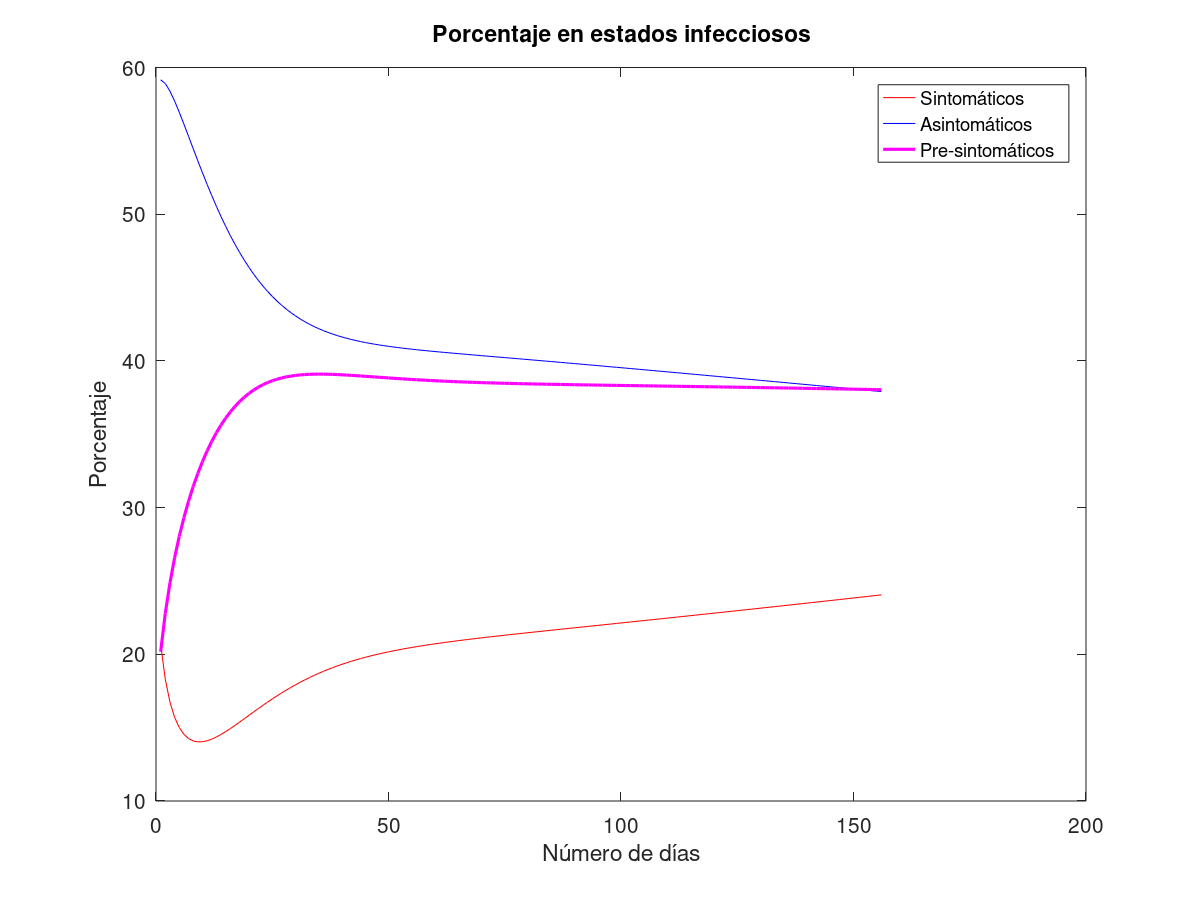
\includegraphics[keepaspectratio, width=12cm]{PorcentajeRespectoInfecciosos.png}
    \caption{\\}
\end{center}  

\begin{center}
    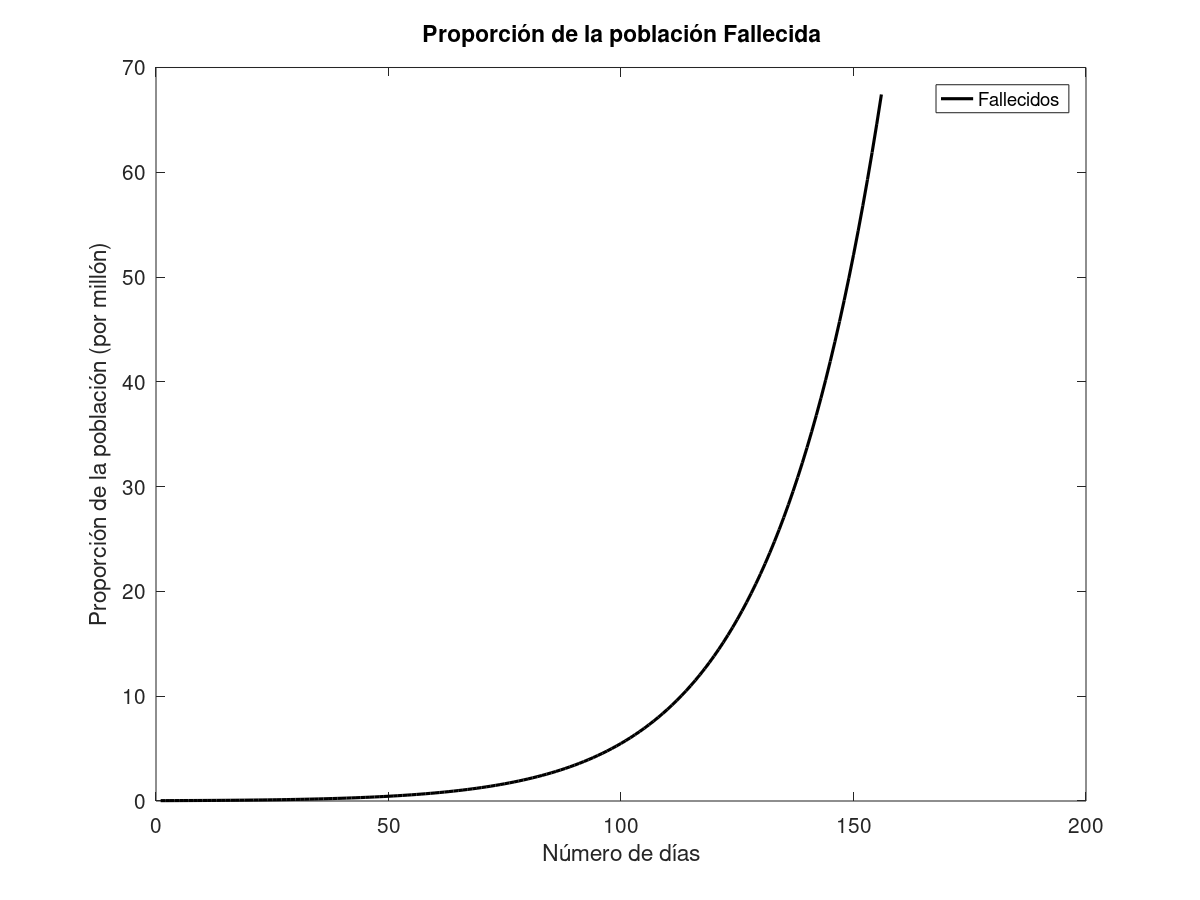
\includegraphics[keepaspectratio, width=12cm]{ProporcionFallecidos.png}
    \caption{\\}
\end{center}  

\begin{center}
    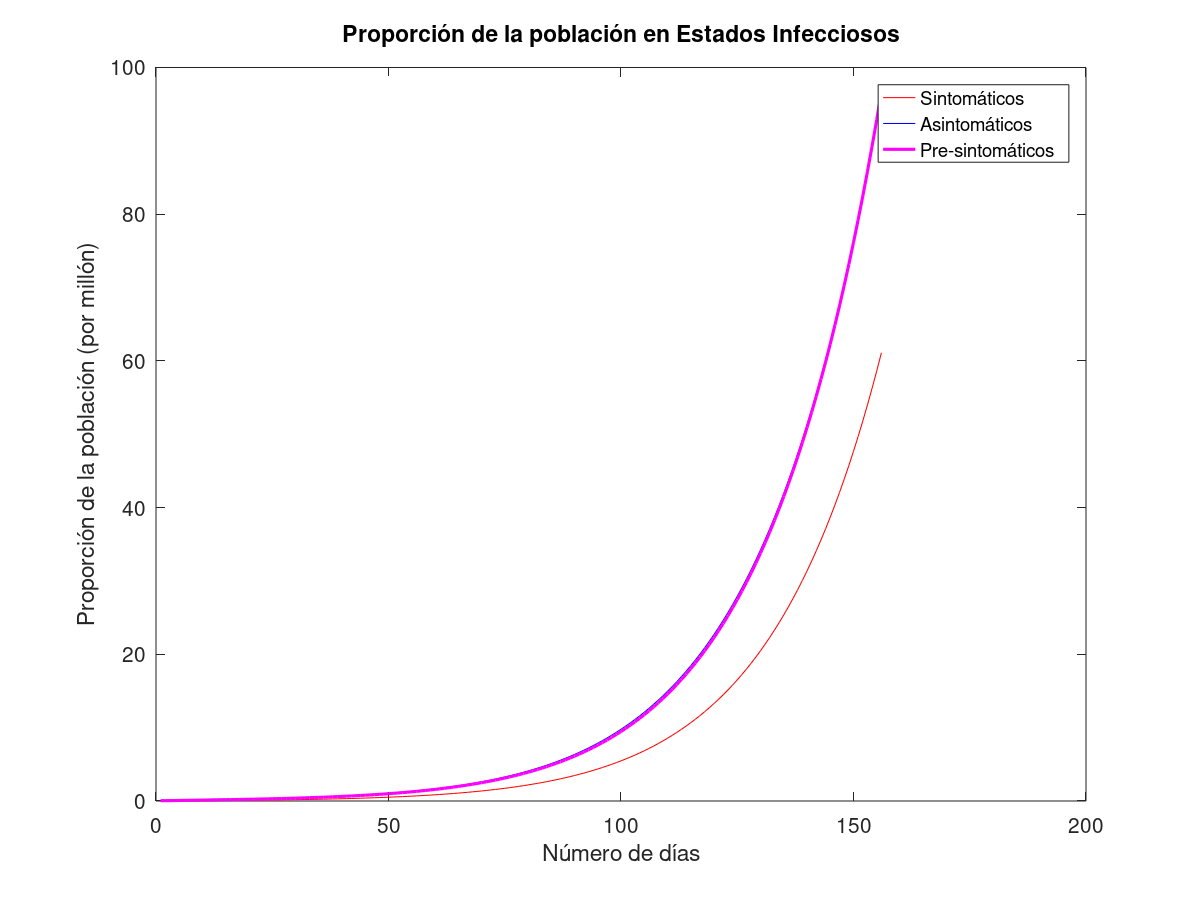
\includegraphics[keepaspectratio, width=12cm]{ProporcionInfecciosos.png}
    \caption{\\}
\end{center}  

\begin{center}
    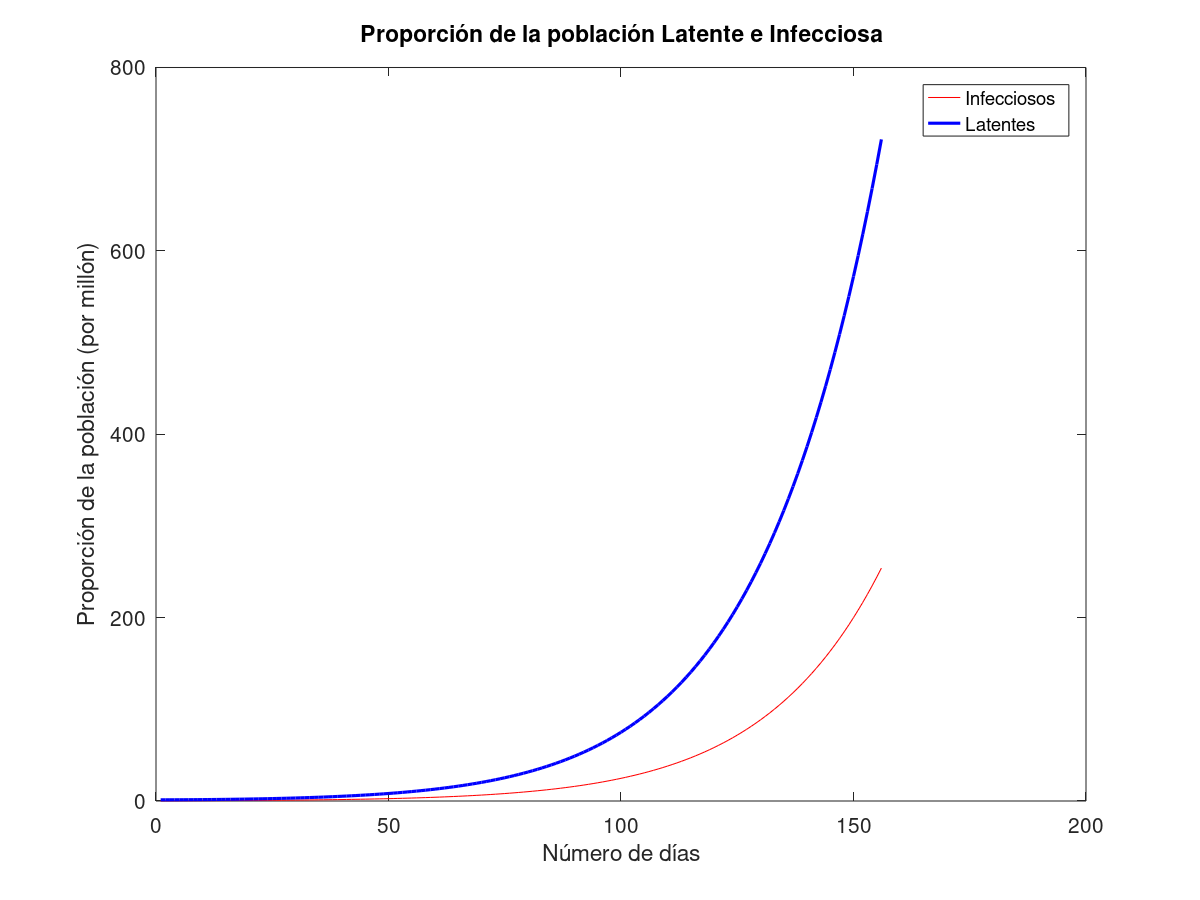
\includegraphics[keepaspectratio, width=12cm]{ProporcionLatentesInfecciosos.png}
    \caption{\\}
\end{center}  

\begin{center}
    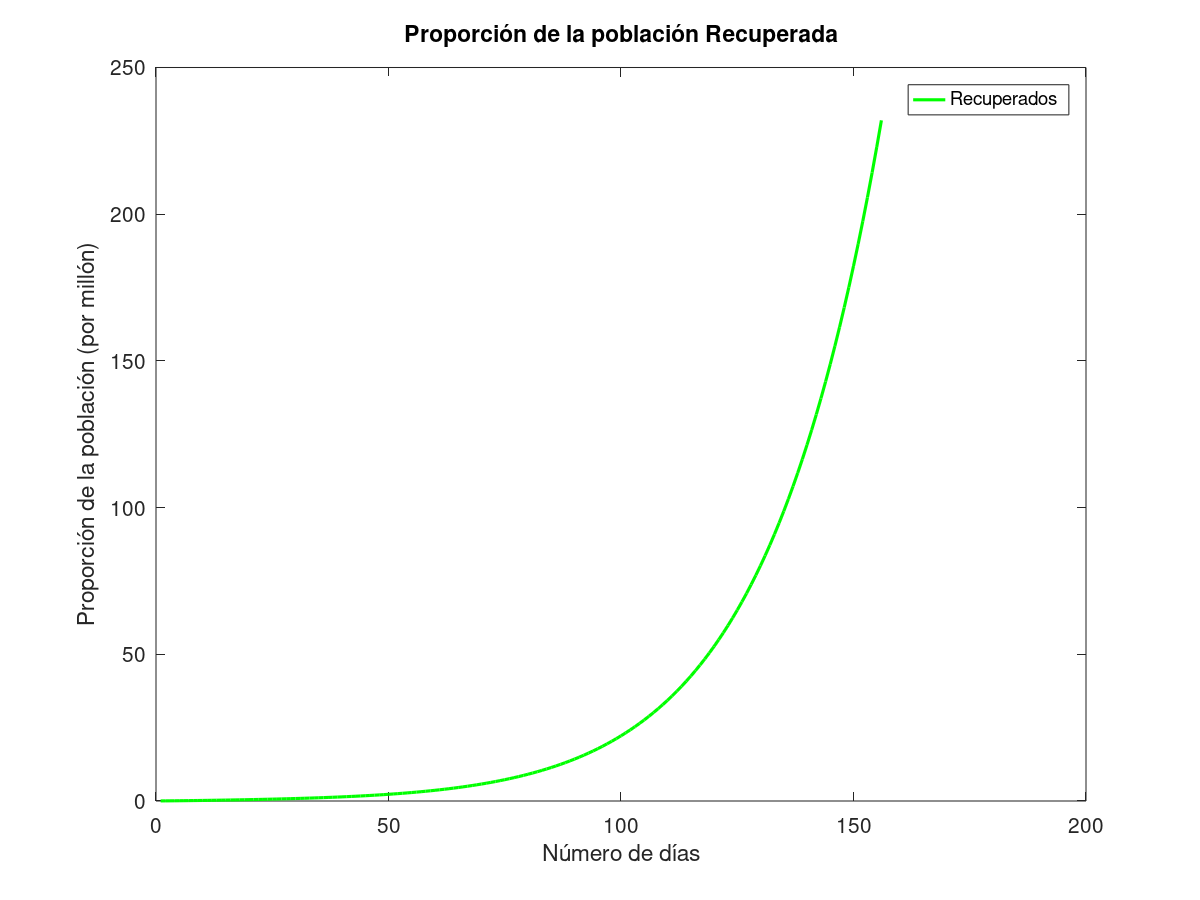
\includegraphics[keepaspectratio, width=12cm]{ProporcionRecuperados.png}
    \caption{\\}
\end{center}  

\begin{center}
    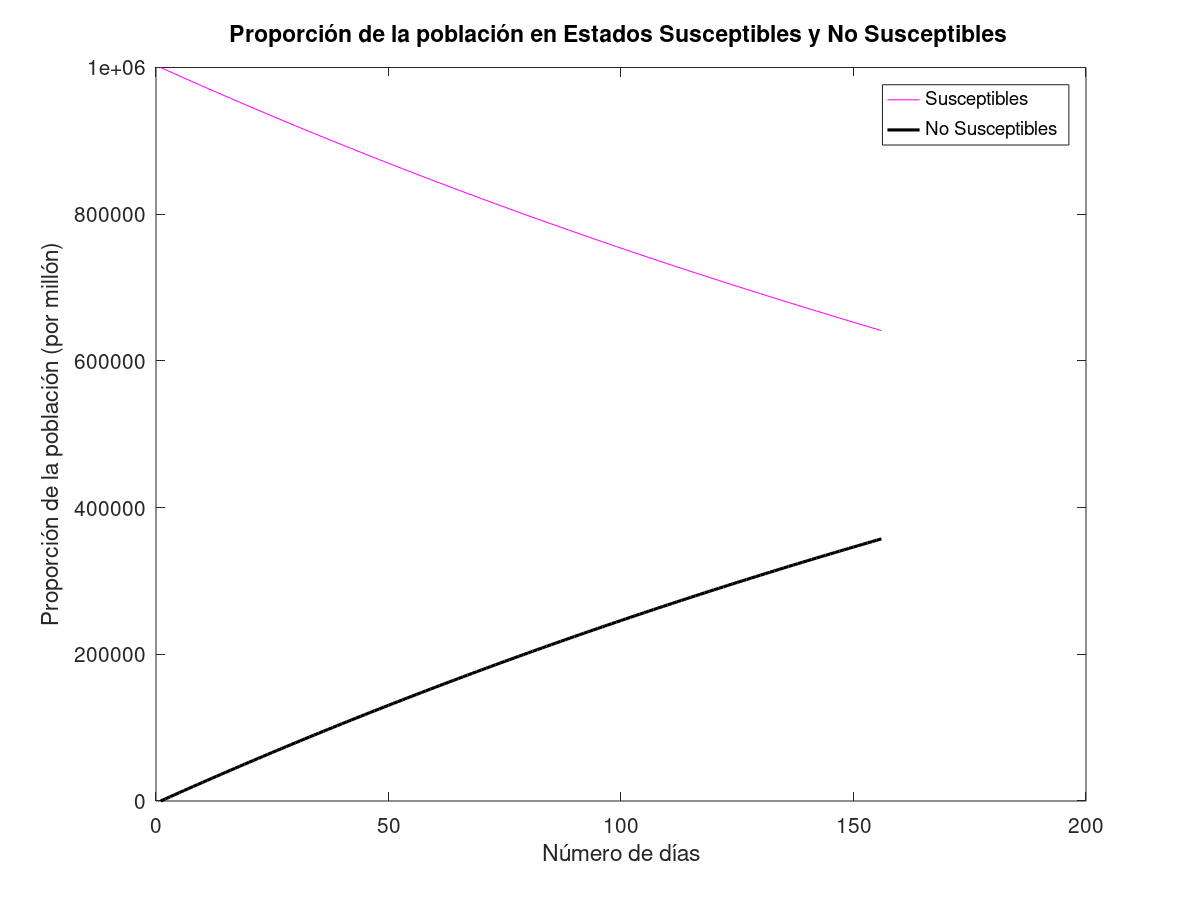
\includegraphics[keepaspectratio, width=12cm]{ProporcionSusceptiblesNoSusceptibles.png}
    \caption{\\}
\end{center}  
\begin{tcolorbox}[colframe=blue!35!black, title=Código]
    CasosAcumulados.m
    \\
    Mortalidad.m
\end{tcolorbox}


\end{document}
